% !TeX program = lualatex
% ALIUS Bulletin native visual reconstruction source.
% Generated from off-repo reference layout data; does not include or input a pre-existing article PDF.
\ifdefined\ALIUSIssueBuild
\else
\documentclass{article}
\usepackage[paperwidth=595.0000bp,paperheight=842.0000bp,margin=0bp]{geometry}
\usepackage{graphicx}
\usepackage{xcolor}
\usepackage{tikz}
\usepackage{iftex}
\usepackage[hidelinks]{hyperref}
\ifPDFTeX
  \usepackage[T1]{fontenc}
  \usepackage[utf8]{inputenc}
  \usepackage{textcomp}
  \usepackage{amssymb}
\else
  \usepackage{fontspec}
\fi
\pagestyle{empty}
\fi
\ifPDFTeX
  \providecommand{\ALIUSDeclareUnicodeFallbacks}{%
    \DeclareUnicodeCharacter{00AC}{\ensuremath{\neg}}%
    \DeclareUnicodeCharacter{00BE}{\ensuremath{\frac{3}{4}}}%
    \DeclareUnicodeCharacter{0101}{\=a}%
    \DeclareUnicodeCharacter{0107}{\'c}%
    \DeclareUnicodeCharacter{012B}{\=\i}%
    \DeclareUnicodeCharacter{0131}{\i}%
    \DeclareUnicodeCharacter{0142}{\l}%
    \DeclareUnicodeCharacter{015B}{\'s}%
    \DeclareUnicodeCharacter{016B}{\=u}%
    \DeclareUnicodeCharacter{025C}{q}%
    \DeclareUnicodeCharacter{0278}{t}%
    \DeclareUnicodeCharacter{02AE}{Th}%
    \DeclareUnicodeCharacter{02B0}{ff}%
    \DeclareUnicodeCharacter{02B4}{ffi}%
    \DeclareUnicodeCharacter{02BE}{ft}%
    \DeclareUnicodeCharacter{02BF}{fi}%
    \DeclareUnicodeCharacter{02C0}{fl}%
    \DeclareUnicodeCharacter{02C1}{fi}%
    \DeclareUnicodeCharacter{02D9}{Th}%
    \DeclareUnicodeCharacter{02EF}{gy}%
    \DeclareUnicodeCharacter{0394}{\ensuremath{\Delta}}%
    \DeclareUnicodeCharacter{03B2}{\ensuremath{\beta}}%
    \DeclareUnicodeCharacter{03BA}{\ensuremath{\kappa}}%
    \DeclareUnicodeCharacter{068D}{-}%
    \DeclareUnicodeCharacter{08BC}{ti}%
    \DeclareUnicodeCharacter{099E}{ti}%
    \DeclareUnicodeCharacter{1E43}{\d{m}}%
    \DeclareUnicodeCharacter{1E47}{\d{n}}%
    \DeclareUnicodeCharacter{1E63}{\d{s}}%
    \DeclareUnicodeCharacter{201C}{``}%
    \DeclareUnicodeCharacter{201D}{''}%
    \DeclareUnicodeCharacter{2260}{\ensuremath{\neq}}%
    \DeclareUnicodeCharacter{25A1}{\ensuremath{\square}}%
  }%
  \ifdefined\ALIUSIssueBuild\else\ALIUSDeclareUnicodeFallbacks\fi
  \providecommand{\ALIUSFontLatoLight}{\fontfamily{lato-LF}\fontseries{l}\selectfont}
  \providecommand{\ALIUSFontLatoRegular}{\fontfamily{lato-LF}\fontseries{m}\selectfont}
  \providecommand{\ALIUSFontLatoItalic}{\fontfamily{lato-LF}\fontseries{m}\itshape}
  \providecommand{\ALIUSFontLatoLightItalic}{\fontfamily{lato-LF}\fontseries{l}\itshape}
  \providecommand{\ALIUSFontCormorantRegular}{\fontfamily{CormorantGaramond-LF}\fontseries{m}\selectfont}
  \providecommand{\ALIUSFontCormorantLight}{\fontfamily{CormorantGaramond-LF}\fontseries{l}\selectfont}
  \providecommand{\ALIUSFontCormorantMedium}{\fontfamily{CormorantGaramond-LF}\fontseries{medium}\selectfont}
  \providecommand{\ALIUSFontCormorantBold}{\fontfamily{CormorantGaramond-LF}\fontseries{b}\selectfont}
  \providecommand{\ALIUSFontCormorantItalic}{\fontfamily{CormorantGaramond-LF}\fontseries{m}\itshape}
  \providecommand{\ALIUSFontTimes}{\fontfamily{ptm}\selectfont}
  \providecommand{\ALIUSFontCalibri}{\fontfamily{phv}\selectfont}
  \providecommand{\ALIUSFontCambria}{\fontfamily{ptm}\selectfont}
  \providecommand{\ALIUSFontSymbolFallback}{\fontfamily{ptm}\selectfont}
\else
  \providecommand{\ALIUSFontLatoLight}{\fontspec{Lato Light}}
  \providecommand{\ALIUSFontLatoRegular}{\fontspec{Lato Regular}}
  \providecommand{\ALIUSFontLatoItalic}{\fontspec{Lato Italic}}
  \providecommand{\ALIUSFontLatoLightItalic}{\fontspec{Lato Light Italic}}
  \providecommand{\ALIUSFontCormorantRegular}{\fontspec{Cormorant Garamond Regular}}
  \providecommand{\ALIUSFontCormorantLight}{\fontspec{Cormorant Garamond Light}}
  \providecommand{\ALIUSFontCormorantMedium}{\fontspec{Cormorant Garamond Medium}}
  \providecommand{\ALIUSFontCormorantBold}{\fontspec{Cormorant Garamond Bold}}
  \providecommand{\ALIUSFontCormorantItalic}{\fontspec{Cormorant Garamond Italic}}
  \providecommand{\ALIUSFontTimes}{\fontspec{Times New Roman}}
  \providecommand{\ALIUSFontCalibri}{\fontspec{Calibri}}
  \providecommand{\ALIUSFontCambria}{\fontspec{Cambria}}
  \providecommand{\ALIUSFontSymbolFallback}{\fontspec{Times New Roman}}
\fi
\providecommand{\ALIUSPullQuoteOpen}{\textquotedblleft}
\providecommand{\ALIUSPullQuoteClose}{\textquotedblright}
\definecolor{ALIUSC000000}{HTML}{000000}
\definecolor{ALIUSC1A1718}{HTML}{1A1718}
\definecolor{ALIUSC1F8135}{HTML}{1F8135}
\definecolor{ALIUSC222222}{HTML}{222222}
\definecolor{ALIUSC595959}{HTML}{595959}
\definecolor{ALIUSC767171}{HTML}{767171}
\definecolor{ALIUSC7F7F7F}{HTML}{7F7F7F}
\definecolor{ALIUSCBFBFBF}{HTML}{BFBFBF}
\definecolor{ALIUSCFFFFFF}{HTML}{FFFFFF}
\providecommand{\ALIUSPlacedText}[6]{%
  \node[anchor=north west,inner sep=0pt,outer sep=0pt,text=#4] at (#1bp,-#2bp) {%
    \resizebox{#3bp}{!}{{#5\fontsize{#6bp}{#6bp}\selectfont #6\kern0pt}}%
  };%
}
\providecommand{\ALIUSPlacedTextContent}[7]{%
  \node[anchor=north west,inner sep=0pt,outer sep=0pt,text=#4] at (#1bp,-#2bp) {%
    \resizebox{#3bp}{!}{{#5\fontsize{#6bp}{#6bp}\selectfont #7}}%
  };%
}
% --- Draft abstract retained as comments; not rendered in reconstruction. ---
% \section*{Abstract}
% This interview with Kevin O'Regan presents the sensorimotor theory of consciousness as a way of dissolving the hard problem by redefining experience. O'Regan lays out the theory in two layers: a top layer of being conscious of something, corresponding to the easy problem, and a bottom layer in which the feel of perceptual experience is constituted by how an animal interacts with the world according to lawful sensorimotor contingencies. He recounts moving from physics into experimental psychology and seeing a logical flaw in the assumption that perception involves an internal representation. The conversation contrasts the sensorimotor theory with the ecological approach of James Gibson, embodied artificial intelligence, autonomous systems, and enactivism, which invoke action but keep a mystery around qualia that need not be there. O'Regan describes the colour work with David Philipona, which predicted which colour names appear most frequently across human languages, and reviews sensory substitution research on seeing with the ears and hearing through the skin, with the adult brain proving less flexible than anticipated. Further sections argue that machines will be conscious to the degree they interact with the world, set consciousness aside as a criterion for ethical decision-making in favour of social agreement, and apply the theory to dreams and hallucinations by holding that the brain enables but does not generate experience, on analogy with vital spirits in biology. The interview closes on O'Regan's next problem, identifying what it is for humans to understand things, set apart from the pattern classification of current machine learning.\par
% --- End draft abstract. ---
\ifdefined\ALIUSIssueBuild
\else
\begin{document}
\fi
% Page 1
\thispagestyle{empty}
\noindent
\begin{tikzpicture}[remember picture,overlay,x=1bp,y=1bp,shift={(current page.north west)}]
  \fill[ALIUSC1F8135] (354.760bp,-172.120bp) rectangle ++(96.720bp,-0.240bp);
  \fill[ALIUSC1F8135] (354.760bp,-232.120bp) rectangle ++(83.760bp,-0.240bp);
  \fill[ALIUSCBFBFBF] (349.000bp,-136.600bp) rectangle ++(0.240bp,-91.920bp);
  \fill[ALIUSCBFBFBF] (349.000bp,-228.520bp) rectangle ++(0.240bp,-2.160bp);
  \fill[ALIUSCBFBFBF] (349.000bp,-230.680bp) rectangle ++(0.240bp,-36.000bp);
  \ALIUSPlacedTextContent{511.620}{35.460}{14.844}{ALIUSC000000}{\ALIUSFontLatoLight}{10.800}{87}
  \ALIUSPlacedTextContent{71.080}{71.099}{198.242}{ALIUSC000000}{\ALIUSFontLatoRegular}{19.920}{On the "feel" of things}
  \ALIUSPlacedTextContent{71.080}{101.311}{325.796}{ALIUSC000000}{\ALIUSFontLatoLight}{17.755}{The sensorimotor theory of consciousness}
  \ALIUSPlacedTextContent{69.640}{136.566}{125.486}{ALIUSC000000}{\ALIUSFontLatoLight}{15.840}{An interview with}
  \ALIUSPlacedTextContent{354.760}{148.740}{73.297}{ALIUSC000000}{\ALIUSFontLatoRegular}{10.800}{Kevin O'Regan}
  \ALIUSPlacedTextContent{69.640}{155.807}{123.329}{ALIUSC000000}{\ALIUSFontLatoLight}{18.960}{Kevin O'Regan}
  \ALIUSPlacedTextContent{354.760}{162.155}{98.502}{ALIUSC1F8135}{\ALIUSFontLatoLight}{8.880}{jkevin.oregan@gmail.com}
  \ALIUSPlacedTextContent{354.760}{172.955}{157.608}{ALIUSC000000}{\ALIUSFontLatoLight}{8.880}{Laboratoire Psychologie de la Perception}
  \ALIUSPlacedTextContent{354.760}{183.755}{133.673}{ALIUSC000000}{\ALIUSFontLatoLight}{8.880}{Université Paris Descartes, France}
  \ALIUSPlacedTextContent{69.640}{190.528}{153.194}{ALIUSC000000}{\ALIUSFontLatoLight}{12.960}{By Cordelia Erickson-Davis}
  \ALIUSPlacedTextContent{354.760}{208.740}{117.857}{ALIUSC000000}{\ALIUSFontLatoRegular}{10.800}{Cordelia Erickson-Davis}
  \ALIUSPlacedTextContent{354.760}{222.155}{85.466}{ALIUSC1F8135}{\ALIUSFontLatoLight}{8.880}{cred22@stanford.edu}
  % ALIUS normalized citation panel begin
  % ALIUS normalized citation panel text: Cite as: O'Regan, K. \& Erickson-Davis, C. (2018). On the "feel" of things: the sensorimotor theory of consciousness. An interview with Kevin O'Regan. ALIUS Bulletin, 2, 87-94.
  \fill[white] (68.140bp,-228.808bp) rectangle ++(278.120bp,-51.300bp);
  \node[anchor=north west,inner sep=0pt,outer sep=0pt,text=ALIUSC000000] at (69.640bp,-230.808bp) {\begin{minipage}{275.120bp}{\ALIUSFontLatoLight\fontsize{9.200bp}{10.700bp}\selectfont\raggedright Cite as: O'Regan, K. \& Erickson-Davis, C. (2018). On the "feel" of things: the sensorimotor theory of consciousness. An interview with Kevin O'Regan. ALIUS Bulletin, 2, 87-94. \mbox{\textcolor{ALIUSC1F8135}{\href{https://doi.org/10.34700/zam3-yk89}{https://doi.org/10.34700/zam3-yk89}}}\par}\end{minipage}};
  % ALIUS normalized citation panel end
  \ALIUSPlacedTextContent{354.760}{232.955}{171.778}{ALIUSC000000}{\ALIUSFontLatoLight}{8.880}{Departments of Anthropology and Medicine}
  \ALIUSPlacedTextContent{354.760}{243.755}{97.242}{ALIUSC000000}{\ALIUSFontLatoLight}{8.880}{Stanford University, USA}
  \ALIUSPlacedTextContent{71.080}{310.288}{455.693}{ALIUSC1F8135}{\ALIUSFontLatoLight}{12.960}{You are primarily interested in the "what it's like" aspect of sensory experience. To}
  \ALIUSPlacedTextContent{71.080}{325.888}{455.809}{ALIUSC1F8135}{\ALIUSFontLatoLight}{12.960}{address it, you've developed what is called the "sensorimotor theory" of}
  \ALIUSPlacedTextContent{71.080}{341.488}{455.842}{ALIUSC1F8135}{\ALIUSFontLatoLight}{12.960}{consciousness (O'Regan \& Noë 2001, Noë \& O'Regan 2002; Myin \& O'Regan 2002,}
  \ALIUSPlacedTextContent{71.080}{357.088}{455.846}{ALIUSC1F8135}{\ALIUSFontLatoLight}{12.960}{O'Regan 2011, O'Regan 2014), which holds perception to be a law-governed mode}
  \ALIUSPlacedTextContent{71.080}{372.688}{455.781}{ALIUSC1F8135}{\ALIUSFontLatoLight}{12.960}{of encounter with the environment. These laws are abstracted from the}
  \ALIUSPlacedTextContent{71.080}{388.288}{455.804}{ALIUSC1F8135}{\ALIUSFontLatoLight}{12.960}{sensorimotor contingencies of the animal in relation with the environment—both}
  \ALIUSPlacedTextContent{71.080}{403.888}{455.867}{ALIUSC1F8135}{\ALIUSFontLatoLight}{12.960}{the contingencies fixed by the perceiver's visual apparatus, as well as those fixed by}
  \ALIUSPlacedTextContent{71.080}{419.488}{455.883}{ALIUSC1F8135}{\ALIUSFontLatoLight}{12.960}{the character of objects. These processes of sensorimotor interaction are distinct}
  \ALIUSPlacedTextContent{71.080}{435.088}{455.857}{ALIUSC1F8135}{\ALIUSFontLatoLight}{12.960}{from perceptual consciousness, however, which you divide into "perceptual}
  \ALIUSPlacedTextContent{71.080}{450.688}{455.842}{ALIUSC1F8135}{\ALIUSFontLatoLight}{12.960}{awareness" on one hand (or "transitive perceptual consciousness"), which is the}
  \ALIUSPlacedTextContent{71.080}{466.288}{455.827}{ALIUSC1F8135}{\ALIUSFontLatoLight}{12.960}{exercise of one's practical knowledge of these sensorimotor contingencies, and}
  \ALIUSPlacedTextContent{71.080}{481.888}{455.819}{ALIUSC1F8135}{\ALIUSFontLatoLight}{12.960}{"general perceptual consciousness" on the other, which is the capacity to become}
  \ALIUSPlacedTextContent{71.080}{497.488}{455.972}{ALIUSC1F8135}{\ALIUSFontLatoLight}{12.960}{aware. Do I have that right? Could you further describe the theory, and in particular}
  \ALIUSPlacedTextContent{71.080}{513.089}{455.959}{ALIUSC1F8135}{\ALIUSFontLatoLight}{12.960}{focus on how it addresses consciousness from the perspective of what you and}
  \ALIUSPlacedTextContent{71.080}{528.688}{409.846}{ALIUSC1F8135}{\ALIUSFontLatoLight}{12.960}{others have described as the "easy" and "hard" problems of consciousness?}
  \ALIUSPlacedTextContent{71.080}{556.218}{456.527}{ALIUSC1A1718}{\ALIUSFontCormorantRegular}{13.920}{Yes, I'd say you've got it more or less right. But the way you say it sounds very}
  \ALIUSPlacedTextContent{71.080}{573.018}{456.753}{ALIUSC1A1718}{\ALIUSFontCormorantRegular}{13.920}{technical. I would have liked you to stress the luminous simplicity of the idea and}
  \ALIUSPlacedTextContent{71.080}{590.058}{314.345}{ALIUSC1A1718}{\ALIUSFontCormorantRegular}{13.920}{why it is a breakthrough in understanding consciousness!}
  \ALIUSPlacedTextContent{71.080}{619.098}{456.470}{ALIUSC1A1718}{\ALIUSFontCormorantRegular}{13.920}{To explain better, let me first note that most people think that consciousness is a}
  \ALIUSPlacedTextContent{71.080}{635.898}{456.660}{ALIUSC1A1718}{\ALIUSFontCormorantRegular}{13.920}{mystery—they think that there is a problem in explaining how physical and chemical}
  \ALIUSPlacedTextContent{71.080}{652.938}{456.431}{ALIUSC1A1718}{\ALIUSFontCormorantRegular}{13.920}{processes in a brain could somehow generate subjective experience. Philosophers call}
  \ALIUSPlacedTextContent{71.080}{669.978}{225.587}{ALIUSC1A1718}{\ALIUSFontCormorantRegular}{13.920}{this the "hard" problem of consciousness.}
  \ALIUSPlacedTextContent{71.080}{698.778}{456.607}{ALIUSC1A1718}{\ALIUSFontCormorantRegular}{13.920}{Science doesn't just advance by making discoveries: it advances by defining terms in}
  \ALIUSPlacedTextContent{71.080}{715.818}{456.384}{ALIUSC1A1718}{\ALIUSFontCormorantRegular}{13.920}{more precise ways. I think such redefining is what's needed to understand}
  \ALIUSPlacedTextContent{71.080}{732.618}{456.532}{ALIUSC1A1718}{\ALIUSFontCormorantRegular}{13.920}{consciousness. The following is a way of defining consciousness that captures what}
  \ALIUSPlacedTextContent{71.080}{749.658}{456.298}{ALIUSC1A1718}{\ALIUSFontCormorantRegular}{13.920}{most people mean by the term, and that at the same time dissolves the mysteries.}
\end{tikzpicture}
\null
\newpage
% Page 2
\thispagestyle{empty}
\noindent
\begin{tikzpicture}[remember picture,overlay,x=1bp,y=1bp,shift={(current page.north west)}]
  \fill[ALIUSC767171] (69.640bp,-54.760bp) rectangle ++(456.480bp,-0.480bp);
  \fill[ALIUSC767171] (69.640bp,-787.000bp) rectangle ++(456.480bp,-0.720bp);
  \ALIUSPlacedTextContent{71.080}{35.460}{165.820}{ALIUSC767171}{\ALIUSFontLatoLight}{10.800}{K. O'Regan – On the "feel" of things}
  \ALIUSPlacedTextContent{511.720}{35.700}{12.644}{ALIUSC767171}{\ALIUSFontLatoLight}{10.800}{88}
  \ALIUSPlacedTextContent{71.080}{70.938}{164.730}{ALIUSC1A1718}{\ALIUSFontCormorantRegular}{13.920}{The definition has two layers:}
  \ALIUSPlacedTextContent{71.080}{99.978}{456.516}{ALIUSC1A1718}{\ALIUSFontCormorantRegular}{13.920}{First, at the top layer: in the normal everyday sense of the word, when you say you}
  \ALIUSPlacedTextContent{71.080}{116.778}{456.600}{ALIUSC1A1718}{\ALIUSFontCormorantRegular}{13.920}{are conscious of something... there has to be a "you" with sufficient cognitive}
  \ALIUSPlacedTextContent{71.080}{133.818}{456.495}{ALIUSC1A1718}{\ALIUSFontCormorantRegular}{13.920}{capacities. People would not normally say of a fly that it is conscious of the cheese it}
  \ALIUSPlacedTextContent{71.080}{150.858}{456.562}{ALIUSC1A1718}{\ALIUSFontCormorantRegular}{13.920}{landed upon: The fly is presumably just a biological machine that is reacting to the}
  \ALIUSPlacedTextContent{71.080}{167.658}{456.654}{ALIUSC1A1718}{\ALIUSFontCormorantRegular}{13.920}{environment. What about the mouse that ate the cheese? And the cat that ate the}
  \ALIUSPlacedTextContent{71.080}{184.698}{456.384}{ALIUSC1A1718}{\ALIUSFontCormorantRegular}{13.920}{mouse? And the dog that chased the cat? And the child that chased the dog? And}
  \ALIUSPlacedTextContent{71.080}{201.738}{456.655}{ALIUSC1A1718}{\ALIUSFontCormorantRegular}{13.920}{the adult that scolded the child? Clearly as we go higher in the hierarchy, we have}
  \ALIUSPlacedTextContent{71.080}{218.538}{456.564}{ALIUSC1A1718}{\ALIUSFontCormorantRegular}{13.920}{higher degrees of being "conscious of". Certainly the adult's, if not the child's,}
  \ALIUSPlacedTextContent{71.080}{235.578}{456.531}{ALIUSC1A1718}{\ALIUSFontCormorantRegular}{13.920}{understanding of the situation involves them not just reacting, but a variety of other}
  \ALIUSPlacedTextContent{71.080}{252.618}{456.577}{ALIUSC1A1718}{\ALIUSFontCormorantRegular}{13.920}{things like knowing that they are reacting, knowing who "they" are, and knowing}
  \ALIUSPlacedTextContent{71.080}{269.418}{411.826}{ALIUSC1A1718}{\ALIUSFontCormorantRegular}{13.920}{why they are reacting, and knowing that they know that they are reacting...}
  \ALIUSPlacedTextContent{71.080}{298.458}{456.478}{ALIUSC1A1718}{\ALIUSFontCormorantRegular}{13.920}{Though maybe too complex for flies and mice, there is nothing magical about such}
  \ALIUSPlacedTextContent{71.080}{315.498}{456.570}{ALIUSC1A1718}{\ALIUSFontCormorantRegular}{13.920}{self-referring cognitive states. Being "conscious of" something in this way is what the}
  \ALIUSPlacedTextContent{71.080}{332.298}{456.535}{ALIUSC1A1718}{\ALIUSFontCormorantRegular}{13.920}{philosophers call the "easy" problem of consciousness. It requires a variety of highly}
  \ALIUSPlacedTextContent{71.080}{349.338}{456.558}{ALIUSC1A1718}{\ALIUSFontCormorantRegular}{13.920}{developed cognitive capacities, including the ability to conceive of one's "self"—but}
  \ALIUSPlacedTextContent{71.080}{366.138}{456.621}{ALIUSC1A1718}{\ALIUSFontCormorantRegular}{13.920}{this mode of being conscious of something is not a mystery. It is coming to my}
  \ALIUSPlacedTextContent{71.080}{383.178}{181.712}{ALIUSC1A1718}{\ALIUSFontCormorantRegular}{13.920}{smartphone in the next decades.}
  \ALIUSPlacedTextContent{71.080}{412.218}{456.682}{ALIUSC1A1718}{\ALIUSFontCormorantRegular}{13.920}{That was the top layer. But now there is the bottom layer of consciousness. I can be}
  \ALIUSPlacedTextContent{71.080}{429.018}{69.639}{ALIUSC1A1718}{\ALIUSFontCormorantRegular}{13.920}{conscious of}
  \ALIUSPlacedTextContent{140.559}{429.018}{65.995}{ALIUSC1A1718}{\ALIUSFontCormorantItalic}{13.920}{an experience}
  \ALIUSPlacedTextContent{206.609}{429.018}{321.052}{ALIUSC1A1718}{\ALIUSFontCormorantRegular}{13.920}{. For example, I can be conscious of the hurt of the pain, or}
  \ALIUSPlacedTextContent{71.080}{446.058}{192.955}{ALIUSC1A1718}{\ALIUSFontCormorantRegular}{13.920}{the redness of a red sunset. They}
  \ALIUSPlacedTextContent{266.249}{446.058}{94.586}{ALIUSC1A1718}{\ALIUSFontCormorantItalic}{13.920}{feel like something}
  \ALIUSPlacedTextContent{360.850}{446.058}{166.804}{ALIUSC1A1718}{\ALIUSFontCormorantRegular}{13.920}{to me. It's not just that I'm}
  \ALIUSPlacedTextContent{71.080}{463.098}{456.555}{ALIUSC1A1718}{\ALIUSFontCormorantRegular}{13.920}{thinking of them or aware of them, like I can think of a pain or of a red sunset. I}
  \ALIUSPlacedTextContent{71.080}{479.898}{45.702}{ALIUSC1A1718}{\ALIUSFontCormorantRegular}{13.920}{actually}
  \ALIUSPlacedTextContent{116.940}{479.898}{16.572}{ALIUSC1A1718}{\ALIUSFontCormorantItalic}{13.920}{feel}
  \ALIUSPlacedTextContent{133.515}{479.898}{394.087}{ALIUSC1A1718}{\ALIUSFontCormorantRegular}{13.920}{them. What is it like to feel things, rather than not feel them like when}
  \ALIUSPlacedTextContent{71.080}{496.938}{456.347}{ALIUSC1A1718}{\ALIUSFontCormorantRegular}{13.920}{you are just thinking about them? This is what the philosophers call the "hard"}
  \ALIUSPlacedTextContent{71.080}{513.978}{456.559}{ALIUSC1A1718}{\ALIUSFontCormorantRegular}{13.920}{problem, or the problem of "qualia". They think it's hard because they see no way}
  \ALIUSPlacedTextContent{71.080}{530.778}{150.199}{ALIUSC1A1718}{\ALIUSFontCormorantRegular}{13.920}{brains could generate feels.}
  \ALIUSPlacedTextContent{140.680}{565.913}{14.160}{ALIUSC7F7F7F}{\ALIUSFontCormorantLight}{48.000}{\ALIUSPullQuoteOpen}
  \ALIUSPlacedTextContent{158.440}{565.913}{281.508}{ALIUSC595959}{\ALIUSFontLatoLight}{14.880}{We should conceive of the feel of a pain, and}
  \ALIUSPlacedTextContent{158.440}{583.913}{288.726}{ALIUSC595959}{\ALIUSFontLatoLight}{14.880}{the feel of red, and all perceptual experiences}
  \ALIUSPlacedTextContent{381.160}{598.648}{14.160}{ALIUSC7F7F7F}{\ALIUSFontCormorantLight}{48.000}{\ALIUSPullQuoteClose}
  \ALIUSPlacedTextContent{158.440}{601.673}{16.558}{ALIUSC595959}{\ALIUSFontLatoLight}{14.880}{as}
  \ALIUSPlacedTextContent{175.000}{601.673}{199.563}{ALIUSC595959}{\ALIUSFontLatoLightItalic}{14.880}{ways of interacting with the world}
  \ALIUSPlacedTextContent{374.680}{601.673}{5.992}{ALIUSC595959}{\ALIUSFontLatoLight}{14.880}{.}
  \ALIUSPlacedTextContent{71.080}{646.698}{456.548}{ALIUSC1A1718}{\ALIUSFontCormorantRegular}{13.920}{And that is where I think a redefinition helps. In fact, the redefinition I propose is}
  \ALIUSPlacedTextContent{71.080}{663.498}{456.583}{ALIUSC1A1718}{\ALIUSFontCormorantRegular}{13.920}{perfectly obvious to the man in the street, who would never imagine that a feel could}
  \ALIUSPlacedTextContent{71.080}{680.538}{456.562}{ALIUSC1A1718}{\ALIUSFontCormorantRegular}{13.920}{be generated by the brain. What after all, is the feel of driving a Porsche? Well, it's}
  \ALIUSPlacedTextContent{71.080}{697.578}{59.647}{ALIUSC1A1718}{\ALIUSFontCormorantRegular}{13.920}{the way it}
  \ALIUSPlacedTextContent{131.991}{697.578}{40.677}{ALIUSC1A1718}{\ALIUSFontCormorantItalic}{13.920}{handles}
  \ALIUSPlacedTextContent{173.947}{697.578}{262.183}{ALIUSC1A1718}{\ALIUSFontCormorantRegular}{13.920}{when you swing around the corner, it's how it}
  \ALIUSPlacedTextContent{437.444}{697.578}{32.105}{ALIUSC1A1718}{\ALIUSFontCormorantItalic}{13.920}{reacts}
  \ALIUSPlacedTextContent{470.818}{697.578}{56.813}{ALIUSC1A1718}{\ALIUSFontCormorantRegular}{13.920}{when you}
  \ALIUSPlacedTextContent{71.080}{714.378}{268.557}{ALIUSC1A1718}{\ALIUSFontCormorantRegular}{13.920}{press the accelerator and it speeds forward... it's}
  \ALIUSPlacedTextContent{340.585}{714.378}{127.026}{ALIUSC1A1718}{\ALIUSFontCormorantItalic}{13.920}{how you interact with it.}
  \ALIUSPlacedTextContent{467.615}{714.378}{60.057}{ALIUSC1A1718}{\ALIUSFontCormorantRegular}{13.920}{Similarly,}
  \ALIUSPlacedTextContent{71.080}{731.418}{456.528}{ALIUSC1A1718}{\ALIUSFontCormorantRegular}{13.920}{we should conceive of the feel of a pain, and the feel of red, and all perceptual}
  \ALIUSPlacedTextContent{71.080}{748.458}{79.862}{ALIUSC1A1718}{\ALIUSFontCormorantRegular}{13.920}{experiences as}
  \ALIUSPlacedTextContent{150.949}{748.458}{177.049}{ALIUSC1A1718}{\ALIUSFontCormorantItalic}{13.920}{ways of interacting with the world.}
  \ALIUSPlacedTextContent{71.080}{793.620}{125.501}{ALIUSC767171}{\ALIUSFontLatoLight}{10.800}{ALIUS Bulletin n°2 (2018)}
  \ALIUSPlacedTextContent{405.163}{793.620}{121.602}{ALIUSC767171}{\ALIUSFontLatoLight}{10.800}{aliusresearch.org/bulletin}
\end{tikzpicture}
\null
\newpage
% Page 3
\thispagestyle{empty}
\noindent
\begin{tikzpicture}[remember picture,overlay,x=1bp,y=1bp,shift={(current page.north west)}]
  \fill[ALIUSC767171] (69.640bp,-54.760bp) rectangle ++(456.480bp,-0.480bp);
  \fill[ALIUSC767171] (69.640bp,-787.000bp) rectangle ++(456.480bp,-0.720bp);
  \ALIUSPlacedTextContent{71.080}{35.460}{165.820}{ALIUSC767171}{\ALIUSFontLatoLight}{10.800}{K. O'Regan – On the "feel" of things}
  \ALIUSPlacedTextContent{511.720}{35.700}{12.644}{ALIUSC767171}{\ALIUSFontLatoLight}{10.800}{89}
  \ALIUSPlacedTextContent{71.080}{70.938}{456.618}{ALIUSC1A1718}{\ALIUSFontCormorantRegular}{13.920}{At first counterintuitive for the scientist looking for brain mechanisms, this way of}
  \ALIUSPlacedTextContent{71.080}{87.978}{456.621}{ALIUSC1A1718}{\ALIUSFontCormorantRegular}{13.920}{thinking about experience provides an exquisitely simple account of the "hard"}
  \ALIUSPlacedTextContent{71.080}{104.778}{456.528}{ALIUSC1A1718}{\ALIUSFontCormorantRegular}{13.920}{problem: when you have an experience, the what-it's-like of the experience is}
  \ALIUSPlacedTextContent{71.080}{121.818}{81.621}{ALIUSC1A1718}{\ALIUSFontCormorantRegular}{13.920}{constituted by}
  \ALIUSPlacedTextContent{152.412}{121.818}{158.424}{ALIUSC1A1718}{\ALIUSFontCormorantItalic}{13.920}{how you interact with the world}
  \ALIUSPlacedTextContent{310.863}{121.818}{216.746}{ALIUSC1A1718}{\ALIUSFontCormorantRegular}{13.920}{when you're having the experience. But}
  \ALIUSPlacedTextContent{71.080}{138.858}{173.776}{ALIUSC1A1718}{\ALIUSFontCormorantRegular}{13.920}{this experienced quality is not}
  \ALIUSPlacedTextContent{246.552}{138.858}{58.575}{ALIUSC1A1718}{\ALIUSFontCormorantItalic}{13.920}{consciously}
  \ALIUSPlacedTextContent{306.857}{138.858}{220.770}{ALIUSC1A1718}{\ALIUSFontCormorantRegular}{13.920}{experienced unless you as a person are}
  \ALIUSPlacedTextContent{71.080}{155.658}{456.568}{ALIUSC1A1718}{\ALIUSFontCormorantRegular}{13.920}{attending to it, making use of it in your rational thoughts, decisions, planning etc.,}
  \ALIUSPlacedTextContent{71.080}{172.698}{444.641}{ALIUSC1A1718}{\ALIUSFontCormorantRegular}{13.920}{in the way of being "conscious of" that I described in the top layer of my account.}
  \ALIUSPlacedTextContent{71.080}{201.738}{456.569}{ALIUSC1A1718}{\ALIUSFontCormorantRegular}{13.920}{In summary: you are having a conscious experience of red when, at the top layer, you}
  \ALIUSPlacedTextContent{71.080}{218.538}{456.537}{ALIUSC1A1718}{\ALIUSFontCormorantRegular}{13.920}{are "conscious of" the fact that, at the bottom layer: you are currently engaged in}
  \ALIUSPlacedTextContent{71.080}{235.578}{456.428}{ALIUSC1A1718}{\ALIUSFontCormorantRegular}{13.920}{interacting with the world in a way that is constitutive of the laws of redness. The}
  \ALIUSPlacedTextContent{71.080}{252.618}{456.557}{ALIUSC1A1718}{\ALIUSFontCormorantRegular}{13.920}{top layer provides the awareness, the bottom layer provides the experienced quality.}
  \ALIUSPlacedTextContent{71.080}{281.488}{455.907}{ALIUSC1F8135}{\ALIUSFontLatoLight}{12.960}{What motivated you to think about these issues, and what was your training up until}
  \ALIUSPlacedTextContent{71.080}{297.088}{61.195}{ALIUSC1F8135}{\ALIUSFontLatoLight}{12.960}{that point?}
  \ALIUSPlacedTextContent{71.080}{324.618}{456.447}{ALIUSC1A1718}{\ALIUSFontCormorantRegular}{13.920}{Ever since I was a child I wanted to make a machine that thinks. I started off studying}
  \ALIUSPlacedTextContent{71.080}{341.658}{456.564}{ALIUSC1A1718}{\ALIUSFontCormorantRegular}{13.920}{physics, because I thought the brain could be understood using the methods of}
  \ALIUSPlacedTextContent{71.080}{358.698}{456.726}{ALIUSC1A1718}{\ALIUSFontCormorantRegular}{13.920}{statistical physics that try to model the behavior of large numbers of interacting}
  \ALIUSPlacedTextContent{71.080}{375.498}{456.573}{ALIUSC1A1718}{\ALIUSFontCormorantRegular}{13.920}{bodies. I then moved into experimental psychology, where I worked on eye}
  \ALIUSPlacedTextContent{71.080}{392.538}{456.556}{ALIUSC1A1718}{\ALIUSFontCormorantRegular}{13.920}{movements and visual perception. I realized that there was a logical flaw in the way}
  \ALIUSPlacedTextContent{71.080}{409.338}{456.494}{ALIUSC1A1718}{\ALIUSFontCormorantRegular}{13.920}{people think about perception: people assume that perception involves the brain}
  \ALIUSPlacedTextContent{71.080}{426.378}{456.487}{ALIUSC1A1718}{\ALIUSFontCormorantRegular}{13.920}{making an internal representation of the world. But then: who or what perceives}
  \ALIUSPlacedTextContent{71.080}{443.418}{456.646}{ALIUSC1A1718}{\ALIUSFontCormorantRegular}{13.920}{that internal representation? It was this realization that led me to postulate a}
  \ALIUSPlacedTextContent{71.080}{460.218}{456.563}{ALIUSC1A1718}{\ALIUSFontCormorantRegular}{13.920}{"sensorimotor" theory, where perceiving involves interacting with the world, not}
  \ALIUSPlacedTextContent{71.080}{477.258}{192.492}{ALIUSC1A1718}{\ALIUSFontCormorantRegular}{13.920}{making an internal representation.}
  \ALIUSPlacedTextContent{71.080}{506.368}{455.925}{ALIUSC1F8135}{\ALIUSFontLatoLight}{12.960}{Many aspects of your theory resonate with other approaches that fall under the}
  \ALIUSPlacedTextContent{71.080}{521.969}{455.787}{ALIUSC1F8135}{\ALIUSFontLatoLight}{12.960}{umbrella of "embodied cognition". This includes the "ecological perspective" of}
  \ALIUSPlacedTextContent{71.080}{537.568}{455.789}{ALIUSC1F8135}{\ALIUSFontLatoLight}{12.960}{Gibson (1966, 1979), the programs of "active" and "animate" perception (Aloimonos}
  \ALIUSPlacedTextContent{71.080}{553.168}{455.845}{ALIUSC1F8135}{\ALIUSFontLatoLight}{12.960}{et al. 1988; Ballard et al. 1997), embodied artificial intelligence (Brooks 1991),}
  \ALIUSPlacedTextContent{71.080}{568.768}{455.972}{ALIUSC1F8135}{\ALIUSFontLatoLight}{12.960}{autonomous systems (Varela \& Bourgine 1992), and enactive perception and}
  \ALIUSPlacedTextContent{71.080}{584.369}{455.800}{ALIUSC1F8135}{\ALIUSFontLatoLight}{12.960}{cognition (Thompson \& Varela 2001; Varela et al. 1991). How does the}
  \ALIUSPlacedTextContent{71.080}{599.969}{313.122}{ALIUSC1F8135}{\ALIUSFontLatoLight}{12.960}{sensorimotor theory compare with these other theories?}
  \ALIUSPlacedTextContent{71.080}{627.498}{456.459}{ALIUSC1A1718}{\ALIUSFontCormorantRegular}{13.920}{The sensorimotor theory is trying to address the "hard" problem of consciousness:}
  \ALIUSPlacedTextContent{71.080}{644.298}{456.536}{ALIUSC1A1718}{\ALIUSFontCormorantRegular}{13.920}{Why do things feel the way they do? Why does "red" look "red" rather than "green".}
  \ALIUSPlacedTextContent{71.080}{661.338}{456.558}{ALIUSC1A1718}{\ALIUSFontCormorantRegular}{13.920}{Why does "red" not sound like a bell? Gibson's ecological approach and embodied}
  \ALIUSPlacedTextContent{71.080}{678.378}{456.409}{ALIUSC1A1718}{\ALIUSFontCormorantRegular}{13.920}{artificial intelligence are not trying to solve that issue, and are instead looking at the}
  \ALIUSPlacedTextContent{71.080}{695.178}{456.604}{ALIUSC1A1718}{\ALIUSFontCormorantRegular}{13.920}{role of action in perception. To me this is not very exciting: action obviously}
  \ALIUSPlacedTextContent{71.080}{712.218}{456.467}{ALIUSC1A1718}{\ALIUSFontCormorantRegular}{13.920}{improves perception because it provides more information to be gathered. But these}
  \ALIUSPlacedTextContent{71.080}{729.258}{456.620}{ALIUSC1A1718}{\ALIUSFontCormorantRegular}{13.920}{approaches miss another important role for action, namely what it brings to an}
  \ALIUSPlacedTextContent{71.080}{746.058}{450.423}{ALIUSC1A1718}{\ALIUSFontCormorantRegular}{13.920}{understanding of the experienced quality of sensory experience and consciousness.}
  \ALIUSPlacedTextContent{71.080}{793.620}{125.501}{ALIUSC767171}{\ALIUSFontLatoLight}{10.800}{ALIUS Bulletin n°2 (2018)}
  \ALIUSPlacedTextContent{405.163}{793.620}{121.602}{ALIUSC767171}{\ALIUSFontLatoLight}{10.800}{aliusresearch.org/bulletin}
\end{tikzpicture}
\null
\newpage
% Page 4
\thispagestyle{empty}
\noindent\begin{tikzpicture}[remember picture,overlay,x=1bp,y=1bp,shift={(current page.north west)}]
  \fill[ALIUSC767171] (69.640bp,-54.760bp) rectangle ++(456.480bp,-0.480bp);
  \fill[ALIUSC767171] (69.640bp,-787.000bp) rectangle ++(456.480bp,-0.720bp);
  \ALIUSPlacedTextContent{71.080}{35.460}{165.820}{ALIUSC767171}{\ALIUSFontLatoLight}{10.800}{K. O'Regan – On the "feel" of things}
  \ALIUSPlacedTextContent{511.720}{35.700}{12.644}{ALIUSC767171}{\ALIUSFontLatoLight}{10.800}{90}
  \ALIUSPlacedTextContent{71.080}{70.938}{456.451}{ALIUSC1A1718}{\ALIUSFontCormorantRegular}{13.920}{Autonomous systems and enactive approaches are, on the other hand, addressing}
  \ALIUSPlacedTextContent{71.080}{87.978}{456.614}{ALIUSC1A1718}{\ALIUSFontCormorantRegular}{13.920}{the issue of consciousness. They invoke action as an essential element in}
  \ALIUSPlacedTextContent{71.080}{104.778}{456.423}{ALIUSC1A1718}{\ALIUSFontCormorantRegular}{13.920}{consciousness. However, my impression is that they think that there is something}
  \ALIUSPlacedTextContent{71.080}{121.818}{456.578}{ALIUSC1A1718}{\ALIUSFontCormorantRegular}{13.920}{magical about action. They think that interaction with the world somehow instills}
  \ALIUSPlacedTextContent{71.080}{138.858}{456.493}{ALIUSC1A1718}{\ALIUSFontCormorantRegular}{13.920}{consciousness into biological systems. Their appeal to interaction, and concepts like}
  \ALIUSPlacedTextContent{71.080}{155.658}{456.445}{ALIUSC1A1718}{\ALIUSFontCormorantRegular}{13.920}{autopoeisis, seems to be an attempt to use mysterious notions to elucidate what they}
  \ALIUSPlacedTextContent{71.080}{172.698}{456.520}{ALIUSC1A1718}{\ALIUSFontCormorantRegular}{13.920}{think is even more mysterious, namely consciousness. What these approaches seem}
  \ALIUSPlacedTextContent{71.080}{189.738}{456.542}{ALIUSC1A1718}{\ALIUSFontCormorantRegular}{13.920}{not to have realized is that if we understand the what-it's-like of perceptual}
  \ALIUSPlacedTextContent{71.080}{206.538}{456.651}{ALIUSC1A1718}{\ALIUSFontCormorantRegular}{13.920}{experience as being constituted by what we do when we interact with the world,}
  \ALIUSPlacedTextContent{71.080}{223.578}{456.714}{ALIUSC1A1718}{\ALIUSFontCormorantRegular}{13.920}{then there is actually no mystery. In other words, autonomous systems and enactive}
  \ALIUSPlacedTextContent{71.080}{240.618}{456.406}{ALIUSC1A1718}{\ALIUSFontCormorantRegular}{13.920}{approaches correctly invoke action, but they don't realize why it is that action solves}
  \ALIUSPlacedTextContent{71.080}{257.418}{456.595}{ALIUSC1A1718}{\ALIUSFontCormorantRegular}{13.920}{the mystery of qualia. They seem to want to keep a mystery where there is no}
  \ALIUSPlacedTextContent{71.080}{274.458}{49.163}{ALIUSC1A1718}{\ALIUSFontCormorantRegular}{13.920}{mystery.}
  \ALIUSPlacedTextContent{81.160}{324.233}{14.160}{ALIUSC7F7F7F}{\ALIUSFontCormorantLight}{48.000}{\ALIUSPullQuoteOpen}
  \ALIUSPlacedTextContent{98.680}{324.233}{409.688}{ALIUSC595959}{\ALIUSFontLatoLight}{14.880}{Autonomous systems and enactive approaches seem not to have}
  \ALIUSPlacedTextContent{98.680}{342.233}{387.839}{ALIUSC595959}{\ALIUSFontLatoLight}{14.880}{realized that if we understand the what-it's-like of perceptual}
  \ALIUSPlacedTextContent{98.680}{360.233}{409.322}{ALIUSC595959}{\ALIUSFontLatoLight}{14.880}{experience as being constituted by what we do when we interact}
  \ALIUSPlacedTextContent{410.440}{373.048}{14.160}{ALIUSC7F7F7F}{\ALIUSFontCormorantLight}{48.000}{\ALIUSPullQuoteClose}
  \ALIUSPlacedTextContent{98.680}{377.993}{309.592}{ALIUSC595959}{\ALIUSFontLatoLight}{14.880}{with the world, then there is actually no mystery.}
  \ALIUSPlacedTextContent{71.080}{428.368}{455.792}{ALIUSC1F8135}{\ALIUSFontLatoLight}{12.960}{In your theory, phenomenological inquiry takes on an entirely tractable tone. As you}
  \ALIUSPlacedTextContent{71.080}{443.968}{455.762}{ALIUSC1F8135}{\ALIUSFontLatoLight}{12.960}{say, "the subject matter of phenomenological reflection is not an ephemeral,}
  \ALIUSPlacedTextContent{71.080}{459.568}{453.293}{ALIUSC1F8135}{\ALIUSFontLatoLight}{12.960}{ineffable, sensation-like momentary occurrence in the mind, but, rather, the real-}
  \ALIUSPlacedTextContent{71.080}{475.168}{455.822}{ALIUSC1F8135}{\ALIUSFontLatoLight}{12.960}{world, temporally extended activity of exploring the environment and the structure}
  \ALIUSPlacedTextContent{71.080}{490.768}{455.749}{ALIUSC1F8135}{\ALIUSFontLatoLight}{12.960}{of sensorimotor contingencies" (O'Regan \& Noë 2001, p. 962). What kinds of}
  \ALIUSPlacedTextContent{71.080}{506.368}{455.889}{ALIUSC1F8135}{\ALIUSFontLatoLight}{12.960}{phenomenological reflection have you utilized in your experimental work? That is,}
  \ALIUSPlacedTextContent{71.080}{521.969}{419.135}{ALIUSC1F8135}{\ALIUSFontLatoLight}{12.960}{how have you operationalized subjective inquiry in your empirical approach?}
  \ALIUSPlacedTextContent{71.080}{549.498}{456.497}{ALIUSC1A1718}{\ALIUSFontCormorantRegular}{13.920}{For example, I'm very proud of the work we did with David Philipona on color.}
  \ALIUSPlacedTextContent{71.080}{566.298}{456.577}{ALIUSC1A1718}{\ALIUSFontCormorantRegular}{13.920}{Color a priori doesn't seem to involve interacting with the environment. But by}
  \ALIUSPlacedTextContent{71.080}{583.338}{456.678}{ALIUSC1A1718}{\ALIUSFontCormorantRegular}{13.920}{taking a sensorimotor approach to color, we were forced to postulate that the}
  \ALIUSPlacedTextContent{71.080}{600.138}{456.539}{ALIUSC1A1718}{\ALIUSFontCormorantRegular}{13.920}{experience of color is necessarily rooted in what happens when you move colored}
  \ALIUSPlacedTextContent{71.080}{617.178}{456.597}{ALIUSC1A1718}{\ALIUSFontCormorantRegular}{13.920}{surfaces around in different lights. This gave a completely new idea about what color}
  \ALIUSPlacedTextContent{71.080}{634.218}{456.545}{ALIUSC1A1718}{\ALIUSFontCormorantRegular}{13.920}{perception is, and made interesting predictions about what it means to be a "pure"}
  \ALIUSPlacedTextContent{71.080}{651.018}{456.723}{ALIUSC1A1718}{\ALIUSFontCormorantRegular}{13.920}{color. We found a surprising link to anthropological data about color naming, where}
  \ALIUSPlacedTextContent{71.080}{668.058}{456.493}{ALIUSC1A1718}{\ALIUSFontCormorantRegular}{13.920}{we accurately predicted which color names should occur most frequently. A simple}
  \ALIUSPlacedTextContent{71.080}{685.098}{456.564}{ALIUSC1A1718}{\ALIUSFontCormorantRegular}{13.920}{philosophical idea, the sensorimotor approach, provided a surprising scientific}
  \ALIUSPlacedTextContent{71.080}{701.898}{63.218}{ALIUSC1A1718}{\ALIUSFontCormorantRegular}{13.920}{prediction.}
  \ALIUSPlacedTextContent{71.080}{731.008}{455.849}{ALIUSC1F8135}{\ALIUSFontLatoLight}{12.960}{As you discuss in your book, the consequence of assuming that experience derives}
  \ALIUSPlacedTextContent{71.080}{746.609}{455.779}{ALIUSC1F8135}{\ALIUSFontLatoLight}{12.960}{from the rules that govern action-related changes in sensory input is that the "feel"}
  \ALIUSPlacedTextContent{71.080}{793.620}{125.501}{ALIUSC767171}{\ALIUSFontLatoLight}{10.800}{ALIUS Bulletin n°2 (2018)}
  \ALIUSPlacedTextContent{405.163}{793.620}{121.602}{ALIUSC767171}{\ALIUSFontLatoLight}{10.800}{aliusresearch.org/bulletin}
\end{tikzpicture}
\null
\newpage
% Page 5
\thispagestyle{empty}
\noindent\begin{tikzpicture}[remember picture,overlay,x=1bp,y=1bp,shift={(current page.north west)}]
  \fill[ALIUSC767171] (69.640bp,-54.760bp) rectangle ++(456.480bp,-0.480bp);
  \fill[ALIUSC767171] (69.640bp,-787.000bp) rectangle ++(456.480bp,-0.720bp);
  \ALIUSPlacedTextContent{71.080}{35.460}{165.820}{ALIUSC767171}{\ALIUSFontLatoLight}{10.800}{K. O'Regan – On the "feel" of things}
  \ALIUSPlacedTextContent{511.720}{35.700}{12.644}{ALIUSC767171}{\ALIUSFontLatoLight}{10.800}{91}
  \ALIUSPlacedTextContent{71.080}{71.008}{455.722}{ALIUSC1F8135}{\ALIUSFontLatoLight}{12.960}{of perceptual modalities like visual experience should be obtainable via channels}
  \ALIUSPlacedTextContent{71.080}{86.609}{455.816}{ALIUSC1F8135}{\ALIUSFontLatoLight}{12.960}{other than vision ("provided that the brain extracts the same invariants from}
  \ALIUSPlacedTextContent{71.080}{102.208}{455.737}{ALIUSC1F8135}{\ALIUSFontLatoLight}{12.960}{structure") (O'Regan \& Noë 2001, p. 956). That is to say: sensory substitution. Can}
  \ALIUSPlacedTextContent{71.080}{117.808}{455.771}{ALIUSC1F8135}{\ALIUSFontLatoLight}{12.960}{you describe the sensory substitution work you've done over the years, and what}
  \ALIUSPlacedTextContent{71.080}{133.408}{127.214}{ALIUSC1F8135}{\ALIUSFontLatoLight}{12.960}{you've learned from it?}
  \ALIUSPlacedTextContent{71.080}{160.938}{456.792}{ALIUSC1A1718}{\ALIUSFontCormorantRegular}{13.920}{Indeed, the sensorimotor theory predicts you should be able to see with your ears,}
  \ALIUSPlacedTextContent{71.080}{177.978}{456.515}{ALIUSC1A1718}{\ALIUSFontCormorantRegular}{13.920}{for example, or hear with your skin, provided you use some technical tricks to}
  \ALIUSPlacedTextContent{71.080}{194.778}{367.630}{ALIUSC1A1718}{\ALIUSFontCormorantRegular}{13.920}{recreate the same sensorimotor laws via alternate sensory channels.}
  \ALIUSPlacedTextContent{71.080}{223.818}{456.480}{ALIUSC1A1718}{\ALIUSFontCormorantRegular}{13.920}{With my collaborators over the last years we have looked at how visual information}
  \ALIUSPlacedTextContent{71.080}{240.858}{456.604}{ALIUSC1A1718}{\ALIUSFontCormorantRegular}{13.920}{can be conveyed through auditory input, how auditory information can be conveyed}
  \ALIUSPlacedTextContent{71.080}{257.658}{456.544}{ALIUSC1A1718}{\ALIUSFontCormorantRegular}{13.920}{through the skin, and how it might be possible to obtain an augmented "sixth" sense}
  \ALIUSPlacedTextContent{71.080}{274.698}{170.554}{ALIUSC1A1718}{\ALIUSFontCormorantRegular}{13.920}{of magnetic North via hearing.}
  \ALIUSPlacedTextContent{71.080}{303.738}{456.609}{ALIUSC1A1718}{\ALIUSFontCormorantRegular}{13.920}{Our efforts have been somewhat disappointing. We have discovered that it is}
  \ALIUSPlacedTextContent{71.080}{320.538}{456.662}{ALIUSC1A1718}{\ALIUSFontCormorantRegular}{13.920}{technically not so easy to provide the brain with the right sensorimotor laws.}
  \ALIUSPlacedTextContent{71.080}{337.578}{456.589}{ALIUSC1A1718}{\ALIUSFontCormorantRegular}{13.920}{Furthermore, we have found that the adult brain seems to be less flexible than we}
  \ALIUSPlacedTextContent{71.080}{354.618}{456.566}{ALIUSC1A1718}{\ALIUSFontCormorantRegular}{13.920}{had thought. Our latest efforts to make a tactile aid that helps hearing-impaired}
  \ALIUSPlacedTextContent{71.080}{371.418}{456.561}{ALIUSC1A1718}{\ALIUSFontCormorantRegular}{13.920}{people better understand speech has proven much more difficult to realize than we}
  \ALIUSPlacedTextContent{71.080}{388.458}{456.491}{ALIUSC1A1718}{\ALIUSFontCormorantRegular}{13.920}{had anticipated. It seems that adult humans have a hard time making the arbitrary}
  \ALIUSPlacedTextContent{71.080}{405.498}{456.692}{ALIUSC1A1718}{\ALIUSFontCormorantRegular}{13.920}{links that we require between speech sounds and tactile patterns. It may be that we}
  \ALIUSPlacedTextContent{71.080}{422.298}{456.628}{ALIUSC1A1718}{\ALIUSFontCormorantRegular}{13.920}{have not been doing things right however. Perhaps the problem is that up until now,}
  \ALIUSPlacedTextContent{71.080}{439.338}{456.498}{ALIUSC1A1718}{\ALIUSFontCormorantRegular}{13.920}{we have not included a proper "action" component in our approach. Sensorimotor}
  \ALIUSPlacedTextContent{71.080}{456.138}{277.513}{ALIUSC1A1718}{\ALIUSFontCormorantRegular}{13.920}{theory would suggest that this would be necessary.}
  \ALIUSPlacedTextContent{133.000}{499.193}{14.160}{ALIUSC7F7F7F}{\ALIUSFontCormorantLight}{48.000}{\ALIUSPullQuoteOpen}
  \ALIUSPlacedTextContent{152.440}{499.193}{291.073}{ALIUSC595959}{\ALIUSFontLatoLight}{14.880}{We will have machines that interact with us in}
  \ALIUSPlacedTextContent{152.440}{517.193}{288.531}{ALIUSC595959}{\ALIUSFontLatoLight}{14.880}{ways that gradually involve higher and higher}
  \ALIUSPlacedTextContent{152.440}{535.193}{308.162}{ALIUSC595959}{\ALIUSFontLatoLight}{14.880}{levels of cognition, including meta-cognition. We}
  \ALIUSPlacedTextContent{152.440}{553.193}{299.272}{ALIUSC595959}{\ALIUSFontLatoLight}{14.880}{will not hesitate to say that they are conscious.}
  \ALIUSPlacedTextContent{452.680}{553.288}{14.160}{ALIUSC7F7F7F}{\ALIUSFontCormorantLight}{48.000}{\ALIUSPullQuoteClose}
  \ALIUSPlacedTextContent{71.080}{601.169}{455.790}{ALIUSC1F8135}{\ALIUSFontLatoLight}{12.960}{You have said you believe that it is possible to build a robot that "feels".  Does that}
  \ALIUSPlacedTextContent{71.080}{616.768}{455.796}{ALIUSC1F8135}{\ALIUSFontLatoLight}{12.960}{mean that you believe artificial intelligence and robots are now or will be considered}
  \ALIUSPlacedTextContent{71.080}{632.369}{61.546}{ALIUSC1F8135}{\ALIUSFontLatoLight}{12.960}{conscious?}
  \ALIUSPlacedTextContent{71.080}{659.898}{456.607}{ALIUSC1A1718}{\ALIUSFontCormorantRegular}{13.920}{Definitely. If consciousness is just a word that describes certain capacities we have}
  \ALIUSPlacedTextContent{71.080}{676.698}{456.694}{ALIUSC1A1718}{\ALIUSFontCormorantRegular}{13.920}{to interact with the world, then machines are already on their way to being}
  \ALIUSPlacedTextContent{71.080}{693.738}{456.490}{ALIUSC1A1718}{\ALIUSFontCormorantRegular}{13.920}{conscious. As I said earlier, whether a mouse, cat, dog, child or adult is conscious is}
  \ALIUSPlacedTextContent{71.080}{710.778}{456.524}{ALIUSC1A1718}{\ALIUSFontCormorantRegular}{13.920}{a matter of degree. Similarly, in the next few decades, we will have machines that}
  \ALIUSPlacedTextContent{71.080}{727.578}{456.459}{ALIUSC1A1718}{\ALIUSFontCormorantRegular}{13.920}{interact with us in ways that gradually involve higher and higher levels of cognition,}
  \ALIUSPlacedTextContent{71.080}{744.618}{456.532}{ALIUSC1A1718}{\ALIUSFontCormorantRegular}{13.920}{including meta-cognition. When such machines interact with us socially every day,}
  \ALIUSPlacedTextContent{71.080}{793.620}{125.501}{ALIUSC767171}{\ALIUSFontLatoLight}{10.800}{ALIUS Bulletin n°2 (2018)}
  \ALIUSPlacedTextContent{405.163}{793.620}{121.602}{ALIUSC767171}{\ALIUSFontLatoLight}{10.800}{aliusresearch.org/bulletin}
\end{tikzpicture}
\null
\newpage
% Page 6
\thispagestyle{empty}
\noindent\begin{tikzpicture}[remember picture,overlay,x=1bp,y=1bp,shift={(current page.north west)}]
  \fill[ALIUSC767171] (69.640bp,-54.760bp) rectangle ++(456.480bp,-0.480bp);
  \fill[ALIUSC767171] (69.640bp,-787.000bp) rectangle ++(456.480bp,-0.720bp);
  \ALIUSPlacedTextContent{71.080}{35.460}{165.820}{ALIUSC767171}{\ALIUSFontLatoLight}{10.800}{K. O'Regan – On the "feel" of things}
  \ALIUSPlacedTextContent{511.720}{35.700}{12.644}{ALIUSC767171}{\ALIUSFontLatoLight}{10.800}{92}
  \ALIUSPlacedTextContent{71.080}{70.938}{456.554}{ALIUSC1A1718}{\ALIUSFontCormorantRegular}{13.920}{when they have levels of knowledge and (meta-)cognition approaching (or}
  \ALIUSPlacedTextContent{71.080}{87.978}{456.541}{ALIUSC1A1718}{\ALIUSFontCormorantRegular}{13.920}{superseding!) ours, we will not hesitate to say that they are conscious. Furthermore,}
  \ALIUSPlacedTextContent{71.080}{104.778}{456.415}{ALIUSC1A1718}{\ALIUSFontCormorantRegular}{13.920}{when machines interact with the world with their senses, they will have experiences}
  \ALIUSPlacedTextContent{71.080}{121.818}{456.558}{ALIUSC1A1718}{\ALIUSFontCormorantRegular}{13.920}{just like we have experiences when we interact with the world. The experiences will}
  \ALIUSPlacedTextContent{71.080}{138.858}{456.544}{ALIUSC1A1718}{\ALIUSFontCormorantRegular}{13.920}{be different of course, precisely to the extent that their modes of interaction are}
  \ALIUSPlacedTextContent{71.080}{155.658}{398.414}{ALIUSC1A1718}{\ALIUSFontCormorantRegular}{13.920}{different from ours. But that is true of mice, cats, dogs, and children too.}
  \ALIUSPlacedTextContent{71.080}{184.768}{455.666}{ALIUSC1F8135}{\ALIUSFontLatoLight}{12.960}{You have also said, in conversation, that you think that our societal focus on}
  \ALIUSPlacedTextContent{71.080}{200.368}{455.807}{ALIUSC1F8135}{\ALIUSFontLatoLight}{12.960}{consciousness as a rubric for ethical decision-making is a mistake. Can you say more}
  \ALIUSPlacedTextContent{71.080}{215.968}{455.842}{ALIUSC1F8135}{\ALIUSFontLatoLight}{12.960}{about this? What kind of ethics of artificial intelligence and other forms of cognitive}
  \ALIUSPlacedTextContent{71.080}{231.568}{455.842}{ALIUSC1F8135}{\ALIUSFontLatoLight}{12.960}{enhancement technologies (e.g., brain machine interface devices) do you think is}
  \ALIUSPlacedTextContent{71.080}{247.169}{48.475}{ALIUSC1F8135}{\ALIUSFontLatoLight}{12.960}{needed?}
  \ALIUSPlacedTextContent{71.080}{274.698}{456.555}{ALIUSC1A1718}{\ALIUSFontCormorantRegular}{13.920}{If consciousness is not an all-or-none thing, and is just a matter of having certain}
  \ALIUSPlacedTextContent{71.080}{291.738}{456.456}{ALIUSC1A1718}{\ALIUSFontCormorantRegular}{13.920}{capacities (and meta-capacities) to interact with the world, then consciousness is}
  \ALIUSPlacedTextContent{71.080}{308.538}{456.582}{ALIUSC1A1718}{\ALIUSFontCormorantRegular}{13.920}{useless as a criterion for ethical decisions. And even if there were some objective}
  \ALIUSPlacedTextContent{71.080}{325.578}{456.543}{ALIUSC1A1718}{\ALIUSFontCormorantRegular}{13.920}{criterion of consciousness, it would be a pretense to invoke it: civilizations have}
  \ALIUSPlacedTextContent{71.080}{342.618}{456.598}{ALIUSC1A1718}{\ALIUSFontCormorantRegular}{13.920}{often denied ethical respect to various perfectly conscious groups. Slaves, women,}
  \ALIUSPlacedTextContent{71.080}{359.418}{456.623}{ALIUSC1A1718}{\ALIUSFontCormorantRegular}{13.920}{certain ethnic and religious groups, have all been denied human rights at various}
  \ALIUSPlacedTextContent{71.080}{376.458}{456.532}{ALIUSC1A1718}{\ALIUSFontCormorantRegular}{13.920}{times through history. Ethics is ultimately a matter of social agreement, and human}
  \ALIUSPlacedTextContent{71.080}{393.498}{456.665}{ALIUSC1A1718}{\ALIUSFontCormorantRegular}{13.920}{societies must take full responsibility for the decisions they take about whom to give}
  \ALIUSPlacedTextContent{71.080}{410.298}{305.484}{ALIUSC1A1718}{\ALIUSFontCormorantRegular}{13.920}{ethical rights to. Appealing to science is just hypocrisy.}
  \ALIUSPlacedTextContent{71.080}{439.408}{453.275}{ALIUSC1F8135}{\ALIUSFontLatoLight}{12.960}{How can sensorimotor theory be applied to "alternative" states if consciousness—}
  \ALIUSPlacedTextContent{71.080}{455.008}{455.731}{ALIUSC1F8135}{\ALIUSFontLatoLight}{12.960}{e.g., dreams and hallucinations? On these perceptual states, you've written that you}
  \ALIUSPlacedTextContent{71.080}{470.608}{455.688}{ALIUSC1F8135}{\ALIUSFontLatoLight}{12.960}{believe them to correspond to implicit knowledge and implicit expectation, based on}
  \ALIUSPlacedTextContent{71.080}{486.208}{455.758}{ALIUSC1F8135}{\ALIUSFontLatoLight}{12.960}{prior perceptual experience. Do you think the study of these states has anything to}
  \ALIUSPlacedTextContent{71.080}{501.808}{388.085}{ALIUSC1F8135}{\ALIUSFontLatoLight}{12.960}{contribute to consciousness studies, from a sensorimotor perspective?}
  \ALIUSPlacedTextContent{71.080}{529.338}{456.555}{ALIUSC1A1718}{\ALIUSFontCormorantRegular}{13.920}{I personally haven't worked on implications of sensorimotor theory for altered states}
  \ALIUSPlacedTextContent{71.080}{546.138}{412.064}{ALIUSC1A1718}{\ALIUSFontCormorantRegular}{13.920}{of consciousness, as produced for example by drugs, trances or meditation.}
  \ALIUSPlacedTextContent{71.080}{575.178}{456.621}{ALIUSC1A1718}{\ALIUSFontCormorantRegular}{13.920}{Note that some critics of sensorimotor theory have claimed that the theory cannot}
  \ALIUSPlacedTextContent{71.080}{592.218}{456.484}{ALIUSC1A1718}{\ALIUSFontCormorantRegular}{13.920}{account for dreams and sensory hallucinations, since these occur without any}
  \ALIUSPlacedTextContent{71.080}{609.018}{456.414}{ALIUSC1A1718}{\ALIUSFontCormorantRegular}{13.920}{interaction with the world. But this is to misunderstand the theory. The theory says}
  \ALIUSPlacedTextContent{71.080}{626.058}{456.498}{ALIUSC1A1718}{\ALIUSFontCormorantRegular}{13.920}{that the quality of an experience resides in what you do when you are interacting}
  \ALIUSPlacedTextContent{71.080}{643.098}{456.462}{ALIUSC1A1718}{\ALIUSFontCormorantRegular}{13.920}{with the world. If, through drugs or dreams you are in the same state that you usually}
  \ALIUSPlacedTextContent{71.080}{659.898}{456.456}{ALIUSC1A1718}{\ALIUSFontCormorantRegular}{13.920}{are in when you are interacting with the world in a "red" way, then you will}
  \ALIUSPlacedTextContent{71.080}{676.938}{451.431}{ALIUSC1A1718}{\ALIUSFontCormorantRegular}{13.920}{experience red, even if now you happen not to be interacting with the world at all.}
  \ALIUSPlacedTextContent{71.080}{705.978}{456.373}{ALIUSC1A1718}{\ALIUSFontCormorantRegular}{13.920}{The critics sometimes go on to say: well, doesn't that show that the brain does}
  \ALIUSPlacedTextContent{71.080}{722.778}{456.448}{ALIUSC1A1718}{\ALIUSFontCormorantRegular}{13.920}{generate experience after all, since you can get the experience without interacting}
  \ALIUSPlacedTextContent{71.080}{739.818}{245.306}{ALIUSC1A1718}{\ALIUSFontCormorantRegular}{13.920}{with the world? My answer is that the brain}
  \ALIUSPlacedTextContent{316.867}{739.818}{35.830}{ALIUSC1A1718}{\ALIUSFontCormorantItalic}{13.920}{enables}
  \ALIUSPlacedTextContent{352.706}{739.818}{174.918}{ALIUSC1A1718}{\ALIUSFontCormorantRegular}{13.920}{the experience, since a brain is}
  \ALIUSPlacedTextContent{71.080}{793.620}{125.501}{ALIUSC767171}{\ALIUSFontLatoLight}{10.800}{ALIUS Bulletin n°2 (2018)}
  \ALIUSPlacedTextContent{405.163}{793.620}{121.602}{ALIUSC767171}{\ALIUSFontLatoLight}{10.800}{aliusresearch.org/bulletin}
\end{tikzpicture}
\null
\newpage
% Page 7
\thispagestyle{empty}
\noindent\begin{tikzpicture}[remember picture,overlay,x=1bp,y=1bp,shift={(current page.north west)}]
  \fill[ALIUSC767171] (69.640bp,-54.760bp) rectangle ++(456.480bp,-0.480bp);
  \fill[ALIUSC767171] (69.640bp,-787.000bp) rectangle ++(456.480bp,-0.720bp);
  \ALIUSPlacedTextContent{71.080}{35.460}{165.820}{ALIUSC767171}{\ALIUSFontLatoLight}{10.800}{K. O'Regan – On the "feel" of things}
  \ALIUSPlacedTextContent{511.720}{35.700}{12.644}{ALIUSC767171}{\ALIUSFontLatoLight}{10.800}{93}
  \ALIUSPlacedTextContent{71.080}{70.938}{456.534}{ALIUSC1A1718}{\ALIUSFontCormorantRegular}{13.920}{necessary in order to interact with the world. But that doesn't mean that the brain}
  \ALIUSPlacedTextContent{71.080}{87.978}{45.415}{ALIUSC1A1718}{\ALIUSFontCormorantItalic}{13.920}{generates}
  \ALIUSPlacedTextContent{116.508}{87.978}{411.205}{ALIUSC1A1718}{\ALIUSFontCormorantRegular}{13.920}{the experience in any meaningful way: Experiences are not the kinds of}
  \ALIUSPlacedTextContent{71.080}{104.778}{456.665}{ALIUSC1A1718}{\ALIUSFontCormorantRegular}{13.920}{things that can be generated. Experiences are modes of interaction with the world.}
  \ALIUSPlacedTextContent{71.080}{121.818}{456.551}{ALIUSC1A1718}{\ALIUSFontCormorantRegular}{13.920}{This new way of thinking about experiences is hard for some people to embrace. But}
  \ALIUSPlacedTextContent{71.080}{138.858}{456.590}{ALIUSC1A1718}{\ALIUSFontCormorantRegular}{13.920}{note that a similar change in point of view happened as regards the notion of life. It}
  \ALIUSPlacedTextContent{71.080}{155.658}{173.462}{ALIUSC1A1718}{\ALIUSFontCormorantRegular}{13.920}{used to be thought that life was}
  \ALIUSPlacedTextContent{244.349}{155.658}{50.694}{ALIUSC1A1718}{\ALIUSFontCormorantItalic}{13.920}{generated}
  \ALIUSPlacedTextContent{294.847}{155.658}{232.766}{ALIUSC1A1718}{\ALIUSFontCormorantRegular}{13.920}{by a vital spirit. Modern biology redefined}
  \ALIUSPlacedTextContent{71.080}{172.698}{456.576}{ALIUSC1A1718}{\ALIUSFontCormorantRegular}{13.920}{our notion of life. It now considers that life is not the kind of thing that is generated.}
  \ALIUSPlacedTextContent{71.080}{189.738}{40.183}{ALIUSC1A1718}{\ALIUSFontCormorantRegular}{13.920}{Life is}
  \ALIUSPlacedTextContent{115.160}{189.738}{37.821}{ALIUSC1A1718}{\ALIUSFontCormorantItalic}{13.920}{enabled}
  \ALIUSPlacedTextContent{153.001}{189.738}{374.638}{ALIUSC1A1718}{\ALIUSFontCormorantRegular}{13.920}{by various physical and chemical mechanisms like respiration,}
  \ALIUSPlacedTextContent{71.080}{206.538}{456.614}{ALIUSC1A1718}{\ALIUSFontCormorantRegular}{13.920}{reproduction, etc. It would be meaningless to say that any one or other such}
  \ALIUSPlacedTextContent{71.080}{223.578}{456.390}{ALIUSC1A1718}{\ALIUSFontCormorantRegular}{13.920}{mechanism "generates" life. Life is a capacity that certain systems have to interact}
  \ALIUSPlacedTextContent{71.080}{240.618}{218.840}{ALIUSC1A1718}{\ALIUSFontCormorantRegular}{13.920}{with the world. Experience is the same.}
  \ALIUSPlacedTextContent{71.080}{269.488}{455.801}{ALIUSC1F8135}{\ALIUSFontLatoLight}{12.960}{What are you spending most of your time thinking about these days, and what's next}
  \ALIUSPlacedTextContent{71.080}{285.088}{46.603}{ALIUSC1F8135}{\ALIUSFontLatoLight}{12.960}{for you?}
  \ALIUSPlacedTextContent{71.080}{312.618}{456.532}{ALIUSC1A1718}{\ALIUSFontCormorantRegular}{13.920}{Modestly, since I think that consciousness is no longer a mystery, I'm trying to solve}
  \ALIUSPlacedTextContent{71.080}{329.658}{456.465}{ALIUSC1A1718}{\ALIUSFontCormorantRegular}{13.920}{a problem that I think is currently a mystery, namely why humans seem to be able}
  \ALIUSPlacedTextContent{71.080}{346.698}{456.559}{ALIUSC1A1718}{\ALIUSFontCormorantRegular}{13.920}{to understand things. Today's machine learning architectures can do good pattern}
  \ALIUSPlacedTextContent{71.080}{363.498}{456.565}{ALIUSC1A1718}{\ALIUSFontCormorantRegular}{13.920}{classification if they are given mounds of examples, but they don't understand what}
  \ALIUSPlacedTextContent{71.080}{380.538}{456.660}{ALIUSC1A1718}{\ALIUSFontCormorantRegular}{13.920}{they're doing. Humans seem to understand things... I'm trying to understand what}
  \ALIUSPlacedTextContent{71.080}{397.338}{106.253}{ALIUSC1A1718}{\ALIUSFontCormorantRegular}{13.920}{it is to understand.}
  \ALIUSPlacedTextContent{71.080}{793.620}{125.501}{ALIUSC767171}{\ALIUSFontLatoLight}{10.800}{ALIUS Bulletin n°2 (2018)}
  \ALIUSPlacedTextContent{405.163}{793.620}{121.602}{ALIUSC767171}{\ALIUSFontLatoLight}{10.800}{aliusresearch.org/bulletin}
\end{tikzpicture}
\null
\newpage
% Page 8
\thispagestyle{empty}
\noindent\begin{tikzpicture}[remember picture,overlay,x=1bp,y=1bp,shift={(current page.north west)}]
  \fill[ALIUSC767171] (69.640bp,-54.760bp) rectangle ++(456.480bp,-0.480bp);
  \fill[ALIUSC767171] (69.640bp,-787.000bp) rectangle ++(456.480bp,-0.720bp);
  \fill[ALIUSCFFFFFF] (71.080bp,-145.000bp) rectangle ++(453.360bp,-15.600bp);
  \fill[ALIUSCFFFFFF] (106.600bp,-160.600bp) rectangle ++(350.160bp,-15.600bp);
  \fill[ALIUSCFFFFFF] (71.080bp,-188.440bp) rectangle ++(453.360bp,-15.600bp);
  \fill[ALIUSCFFFFFF] (106.600bp,-204.280bp) rectangle ++(199.200bp,-15.600bp);
  \fill[ALIUSCFFFFFF] (71.080bp,-231.880bp) rectangle ++(453.360bp,-15.600bp);
  \fill[ALIUSCFFFFFF] (106.600bp,-247.720bp) rectangle ++(18.240bp,-15.600bp);
  \fill[ALIUSCFFFFFF] (71.080bp,-275.320bp) rectangle ++(323.520bp,-15.600bp);
  \fill[ALIUSCFFFFFF] (71.080bp,-303.160bp) rectangle ++(453.360bp,-15.600bp);
  \fill[ALIUSCFFFFFF] (71.080bp,-331.000bp) rectangle ++(453.360bp,-15.600bp);
  \fill[ALIUSCFFFFFF] (106.600bp,-346.600bp) rectangle ++(287.520bp,-15.600bp);
  \fill[ALIUSCFFFFFF] (71.080bp,-374.440bp) rectangle ++(453.360bp,-15.600bp);
  \fill[ALIUSCFFFFFF] (106.600bp,-390.040bp) rectangle ++(417.840bp,-15.600bp);
  \fill[ALIUSCFFFFFF] (106.600bp,-405.880bp) rectangle ++(29.520bp,-15.600bp);
  \fill[ALIUSCFFFFFF] (71.080bp,-433.720bp) rectangle ++(453.360bp,-15.600bp);
  \fill[ALIUSCFFFFFF] (106.600bp,-449.320bp) rectangle ++(395.520bp,-15.600bp);
  \fill[ALIUSCFFFFFF] (71.080bp,-477.160bp) rectangle ++(453.360bp,-15.600bp);
  \fill[ALIUSCFFFFFF] (106.600bp,-492.760bp) rectangle ++(124.800bp,-15.600bp);
  \fill[ALIUSCFFFFFF] (71.080bp,-520.600bp) rectangle ++(453.360bp,-15.600bp);
  \fill[ALIUSCFFFFFF] (106.600bp,-536.440bp) rectangle ++(415.920bp,-15.600bp);
  \fill[ALIUSCFFFFFF] (71.080bp,-564.040bp) rectangle ++(453.360bp,-15.600bp);
  \fill[ALIUSCFFFFFF] (106.600bp,-579.880bp) rectangle ++(276.240bp,-15.600bp);
  \fill[ALIUSCFFFFFF] (71.080bp,-607.480bp) rectangle ++(453.360bp,-15.600bp);
  \fill[ALIUSCFFFFFF] (106.600bp,-623.320bp) rectangle ++(291.120bp,-15.600bp);
  \fill[ALIUSCFFFFFF] (71.080bp,-651.160bp) rectangle ++(453.360bp,-15.600bp);
  \fill[ALIUSCFFFFFF] (106.600bp,-666.760bp) rectangle ++(142.080bp,-15.600bp);
  \ALIUSPlacedTextContent{71.080}{35.460}{165.820}{ALIUSC767171}{\ALIUSFontLatoLight}{10.800}{K. O'Regan – On the "feel" of things}
  \ALIUSPlacedTextContent{511.720}{35.700}{12.644}{ALIUSC767171}{\ALIUSFontLatoLight}{10.800}{94}
  \ALIUSPlacedTextContent{263.991}{71.444}{70.165}{ALIUSC000000}{\ALIUSFontLatoLight}{13.731}{References}
  \ALIUSPlacedTextContent{71.080}{101.585}{340.123}{ALIUSC1A1718}{\ALIUSFontCormorantRegular}{12.960}{Aloimonos, J., Weiss, I., Bandyopadhyay, A. (1988). Active vision.}
  \ALIUSPlacedTextContent{412.188}{101.585}{115.157}{ALIUSC1A1718}{\ALIUSFontCormorantItalic}{12.960}{International Journal of}
  \ALIUSPlacedTextContent{106.530}{117.185}{80.521}{ALIUSC1A1718}{\ALIUSFontCormorantItalic}{12.960}{Computer Vision.}
  \ALIUSPlacedTextContent{187.076}{117.185}{68.629}{ALIUSC1A1718}{\ALIUSFontCormorantRegular}{12.960}{1(4), 333-356.}
  \ALIUSPlacedTextContent{71.080}{145.025}{456.376}{ALIUSC222222}{\ALIUSFontCormorantRegular}{12.960}{Ballard, D. H., Hayhoe, M. M., Pook, P. K., \& Rao, R. P. (1997). Deictic codes for the}
  \ALIUSPlacedTextContent{106.530}{160.625}{135.045}{ALIUSC222222}{\ALIUSFontCormorantRegular}{12.960}{embodiment of cognition.}
  \ALIUSPlacedTextContent{241.585}{160.625}{139.628}{ALIUSC222222}{\ALIUSFontCormorantItalic}{12.960}{Behavioral and Brain Sciences}
  \ALIUSPlacedTextContent{381.241}{160.625}{5.919}{ALIUSC222222}{\ALIUSFontCormorantRegular}{12.960}{,}
  \ALIUSPlacedTextContent{387.169}{160.625}{10.408}{ALIUSC222222}{\ALIUSFontCormorantItalic}{12.960}{20}
  \ALIUSPlacedTextContent{397.594}{160.625}{59.127}{ALIUSC222222}{\ALIUSFontCormorantRegular}{12.960}{(4), 723-742.}
  \ALIUSPlacedTextContent{71.080}{188.465}{399.961}{ALIUSC222222}{\ALIUSFontCormorantRegular}{12.960}{Braund, M. J. (2008). The structures of perception: An ecological perspective.}
  \ALIUSPlacedTextContent{471.839}{188.465}{55.570}{ALIUSC222222}{\ALIUSFontCormorantItalic}{12.960}{Kritike: An}
  \ALIUSPlacedTextContent{106.530}{204.305}{132.840}{ALIUSC222222}{\ALIUSFontCormorantItalic}{12.960}{Online Journal of Philosophy}
  \ALIUSPlacedTextContent{239.412}{204.305}{5.919}{ALIUSC222222}{\ALIUSFontCormorantRegular}{12.960}{,}
  \ALIUSPlacedTextContent{245.340}{204.305}{4.704}{ALIUSC222222}{\ALIUSFontCormorantItalic}{12.960}{2}
  \ALIUSPlacedTextContent{250.059}{204.305}{55.686}{ALIUSC222222}{\ALIUSFontCormorantRegular}{12.960}{(1), 123-144.}
  \ALIUSPlacedTextContent{71.080}{231.905}{291.699}{ALIUSC222222}{\ALIUSFontCormorantRegular}{12.960}{Brooks, R. A. (1991). Intelligence without representation.}
  \ALIUSPlacedTextContent{363.108}{231.905}{96.975}{ALIUSC222222}{\ALIUSFontCormorantItalic}{12.960}{Artificial intelligence}
  \ALIUSPlacedTextContent{460.107}{231.905}{5.919}{ALIUSC222222}{\ALIUSFontCormorantRegular}{12.960}{,}
  \ALIUSPlacedTextContent{466.355}{231.905}{10.514}{ALIUSC222222}{\ALIUSFontCormorantItalic}{12.960}{47}
  \ALIUSPlacedTextContent{476.884}{231.905}{47.483}{ALIUSC222222}{\ALIUSFontCormorantRegular}{12.960}{(1-3), 139-}
  \ALIUSPlacedTextContent{106.530}{247.745}{18.235}{ALIUSC222222}{\ALIUSFontCormorantRegular}{12.960}{159.}
  \ALIUSPlacedTextContent{71.080}{275.345}{323.423}{ALIUSC222222}{\ALIUSFontCormorantRegular}{12.960}{Gibson, J. J. (1966). The senses considered as perceptual systems.}
  \ALIUSPlacedTextContent{71.080}{303.185}{95.655}{ALIUSC222222}{\ALIUSFontCormorantRegular}{12.960}{Gibson, J. J. (2014).}
  \ALIUSPlacedTextContent{166.112}{303.185}{266.056}{ALIUSC222222}{\ALIUSFontCormorantItalic}{12.960}{The ecological approach to visual perception: classic edition}
  \ALIUSPlacedTextContent{432.308}{303.185}{92.065}{ALIUSC222222}{\ALIUSFontCormorantRegular}{12.960}{. Psychology Press.}
  \ALIUSPlacedTextContent{71.080}{331.025}{456.401}{ALIUSC222222}{\ALIUSFontCormorantRegular}{12.960}{O'Regan, J. K., \& Noë, A. (2001). A sensorimotor account of vision and visual}
  \ALIUSPlacedTextContent{106.530}{346.625}{75.025}{ALIUSC222222}{\ALIUSFontCormorantRegular}{12.960}{consciousness.}
  \ALIUSPlacedTextContent{181.564}{346.625}{136.427}{ALIUSC222222}{\ALIUSFontCormorantItalic}{12.960}{Behavioral and brain sciences}
  \ALIUSPlacedTextContent{318.022}{346.625}{5.919}{ALIUSC222222}{\ALIUSFontCormorantRegular}{12.960}{,}
  \ALIUSPlacedTextContent{323.950}{346.625}{10.201}{ALIUSC222222}{\ALIUSFontCormorantItalic}{12.960}{24}
  \ALIUSPlacedTextContent{334.168}{346.625}{59.898}{ALIUSC222222}{\ALIUSFontCormorantRegular}{12.960}{(5), 939-973.}
  \ALIUSPlacedTextContent{71.080}{374.465}{456.340}{ALIUSC222222}{\ALIUSFontCormorantRegular}{12.960}{Myin, E., \& O'Regan, J. K. (2002). Perceptual consciousness, access to modality and skill}
  \ALIUSPlacedTextContent{106.530}{390.065}{239.255}{ALIUSC222222}{\ALIUSFontCormorantRegular}{12.960}{theories. A way to naturalize phenomenology?}
  \ALIUSPlacedTextContent{346.336}{390.065}{150.749}{ALIUSC222222}{\ALIUSFontCormorantItalic}{12.960}{Journal of Consciousness Studies}
  \ALIUSPlacedTextContent{497.171}{390.065}{5.919}{ALIUSC222222}{\ALIUSFontCormorantRegular}{12.960}{,}
  \ALIUSPlacedTextContent{503.685}{390.065}{5.443}{ALIUSC222222}{\ALIUSFontCormorantItalic}{12.960}{9}
  \ALIUSPlacedTextContent{509.145}{390.065}{18.268}{ALIUSC222222}{\ALIUSFontCormorantRegular}{12.960}{(1),}
  \ALIUSPlacedTextContent{106.530}{405.905}{29.476}{ALIUSC222222}{\ALIUSFontCormorantRegular}{12.960}{27-46.}
  \ALIUSPlacedTextContent{71.080}{433.745}{456.318}{ALIUSC222222}{\ALIUSFontCormorantRegular}{12.960}{Noë, A., \& O'Regan, J. K. (2002). On the brain-basis of visual consciousness: A sensorimotor}
  \ALIUSPlacedTextContent{106.530}{449.345}{45.503}{ALIUSC222222}{\ALIUSFontCormorantRegular}{12.960}{account.}
  \ALIUSPlacedTextContent{152.042}{449.345}{302.694}{ALIUSC222222}{\ALIUSFontCormorantItalic}{12.960}{Vision and mind: Selected readings in the philosophy of perception}
  \ALIUSPlacedTextContent{454.779}{449.345}{47.347}{ALIUSC222222}{\ALIUSFontCormorantRegular}{12.960}{, 567-598.}
  \ALIUSPlacedTextContent{71.080}{477.185}{108.918}{ALIUSC222222}{\ALIUSFontCormorantRegular}{12.960}{O'Regan, J. K. (2011).}
  \ALIUSPlacedTextContent{180.480}{477.185}{341.373}{ALIUSC222222}{\ALIUSFontCormorantItalic}{12.960}{Why red doesn't sound like a bell: Understanding the feel of consciousness}
  \ALIUSPlacedTextContent{521.806}{477.185}{5.607}{ALIUSC222222}{\ALIUSFontCormorantRegular}{12.960}{.}
  \ALIUSPlacedTextContent{106.530}{492.785}{124.778}{ALIUSC222222}{\ALIUSFontCormorantRegular}{12.960}{Oxford University Press.}
  \ALIUSPlacedTextContent{71.080}{520.625}{456.310}{ALIUSC222222}{\ALIUSFontCormorantRegular}{12.960}{O'Regan, J. K. (2014). The explanatory status of the sensorimotor approach to phenomenal}
  \ALIUSPlacedTextContent{106.530}{536.465}{216.280}{ALIUSC222222}{\ALIUSFontCormorantRegular}{12.960}{consciousness, and its appeal to cognition.}
  \ALIUSPlacedTextContent{322.819}{536.465}{166.145}{ALIUSC222222}{\ALIUSFontCormorantItalic}{12.960}{Contemporary Sensorimotor Theory}
  \ALIUSPlacedTextContent{489.033}{536.465}{5.919}{ALIUSC222222}{\ALIUSFontCormorantRegular}{12.960}{,}
  \ALIUSPlacedTextContent{494.961}{536.465}{8.630}{ALIUSC222222}{\ALIUSFontCormorantItalic}{12.960}{15}
  \ALIUSPlacedTextContent{503.606}{536.465}{18.802}{ALIUSC222222}{\ALIUSFontCormorantRegular}{12.960}{, 23.}
  \ALIUSPlacedTextContent{71.080}{564.065}{456.296}{ALIUSC222222}{\ALIUSFontCormorantRegular}{12.960}{Thompson, E., \& Varela, F. J. (2001). Radical embodiment: neural dynamics and}
  \ALIUSPlacedTextContent{106.530}{579.905}{75.025}{ALIUSC222222}{\ALIUSFontCormorantRegular}{12.960}{consciousness.}
  \ALIUSPlacedTextContent{181.564}{579.905}{126.275}{ALIUSC222222}{\ALIUSFontCormorantItalic}{12.960}{Trends in cognitive sciences}
  \ALIUSPlacedTextContent{307.830}{579.905}{5.919}{ALIUSC222222}{\ALIUSFontCormorantRegular}{12.960}{,}
  \ALIUSPlacedTextContent{313.758}{579.905}{4.847}{ALIUSC222222}{\ALIUSFontCormorantItalic}{12.960}{5}
  \ALIUSPlacedTextContent{318.620}{579.905}{64.189}{ALIUSC222222}{\ALIUSFontCormorantRegular}{12.960}{(10), 418-425.}
  \ALIUSPlacedTextContent{71.080}{607.505}{206.082}{ALIUSC222222}{\ALIUSFontCormorantRegular}{12.960}{Varela, F. J., \& Bourgine, P. (Eds.). (1992).}
  \ALIUSPlacedTextContent{276.610}{607.505}{250.742}{ALIUSC222222}{\ALIUSFontCormorantItalic}{12.960}{Toward a practice of autonomous systems: Proceedings}
  \ALIUSPlacedTextContent{106.530}{623.345}{231.090}{ALIUSC222222}{\ALIUSFontCormorantItalic}{12.960}{of the First European Conference on Artificial Life}
  \ALIUSPlacedTextContent{337.626}{623.345}{60.079}{ALIUSC222222}{\ALIUSFontCormorantRegular}{12.960}{. MIT press.}
  \ALIUSPlacedTextContent{71.080}{651.185}{249.058}{ALIUSC222222}{\ALIUSFontCormorantRegular}{12.960}{Varela, F. J., Thompson, E., \& Rosch, E. (2017).}
  \ALIUSPlacedTextContent{321.667}{651.185}{205.738}{ALIUSC222222}{\ALIUSFontCormorantItalic}{12.960}{The embodied mind: Cognitive science and}
  \ALIUSPlacedTextContent{106.530}{666.785}{82.166}{ALIUSC222222}{\ALIUSFontCormorantItalic}{12.960}{human experience}
  \ALIUSPlacedTextContent{188.688}{666.785}{60.079}{ALIUSC222222}{\ALIUSFontCormorantRegular}{12.960}{. MIT press.}
  \ALIUSPlacedTextContent{71.080}{793.620}{125.501}{ALIUSC767171}{\ALIUSFontLatoLight}{10.800}{ALIUS Bulletin n°2 (2018)}
  \ALIUSPlacedTextContent{405.163}{793.620}{121.602}{ALIUSC767171}{\ALIUSFontLatoLight}{10.800}{aliusresearch.org/bulletin}
\end{tikzpicture}
\null
\ifdefined\ALIUSIssueBuild
\clearpage
\expandafter\endinput
\fi
\end{document}
